\documentclass{article}      % Specifies the document class
\usepackage[margin=1in]{geometry}
\usepackage{caption}
\usepackage[final]{graphicx}
\usepackage{amsmath}
\usepackage{placeins}
\usepackage{float}           % Add float package for [H] option
\usepackage[T1]{fontenc}
\usepackage{url}
\usepackage{booktabs}
\usepackage[table]{xcolor}
\usepackage{array}
\usepackage{colortbl}
\usepackage{rotating}

\definecolor{lightgray}{gray}{0.7}
\title{Case Study 5: Predicting Firewall Actions Using Support Vector Machines and Stochastic Gradient Descent}
\author{Kristin Henderson}
\date{July 6, 2025}         % Deleting this command produces today's date.

\newcommand{\ip}[2]{(#1, #2)}
                             % Defines \ip{arg1}{arg2} to mean
                             % (arg1, arg2).
                             
\begin{document}             % End of preamble and beginning of text.

\maketitle                   % Produces the title.

\section{Introduction}       % Produces section heading.  Lower-level
                             % sections are begun with similar
                             % \subsection and \subsubsection commands.

This study aims to predict network traffic actions using three classification models: a linear support vector machine (SVM), an SVM with a radial basis function (RBF) kernel, and a logistic regression model trained using stochastic gradient descent (SGD). A well-performing model that balances accuracy and speed could assist in filtering incoming network connection requests, supporting cybersecurity and firewall operations.

\section{Data}

\subsection{Dataset}

The Internet Firewall dataset used in this analysis comes from the University of California Irvine Machine Learning Repository. It contains 65,532 records of network traffic observed at a university firewall. Each record includes 11 features: 4 categorical features indicating port roles and 7 numerical features related to information flow. The multi-class target variable, \texttt{Action}, indicates the firewall's decision: \texttt{allow}, \texttt{drop}, \texttt{deny}, or \texttt{reset-both}. The features are summarized in Table~\ref{table:features}.

\begin{table}[!h]
    \centering
    \caption{Features Used in the Classification Models}
    \small  % or \footnotesize for even smaller
    \begin{tabular}{lp{10cm}}
    \arrayrulecolor{black}  % Start with black rules
    \toprule
    \textbf{Feature} & \textbf{Description} \\
    \midrule
    \arrayrulecolor{lightgray}
    Source Port           & Port number of the originating device \\ \hline
    Destination Port      & Port number of the destination device \\ \hline
    NAT Source Port       & Translated source port through Network Address Translation (NAT) \\ \hline
    NAT Destination Port  & Translated destination port through NAT \\ \hline
    Bytes                 & Total bytes transmitted during the session \\ \hline
    Bytes Sent            & Number of bytes sent from source to destination \\ \hline
    Bytes Received        & Number of bytes received from destination \\ \hline
    Packets               & Total number of packets in the session \\ \hline
    Elapsed Time (sec)    & Duration of the session in seconds \\ \hline
    pkts\_sent            & Number of packets sent \\ \hline
    pkts\_received        & Number of packets received \\ \hline
    Action                & Target: Firewall decision.  Possible values include: \\
    & \textit{allow} (connection permitted) \\
    & \textit{deny} (initial connection blocked) \\
    & \textit{drop} (packets silently discarded) \\
    & \textit{reset-both} (TCP session terminated from both source and destination) \\   
    \arrayrulecolor{black}
    \bottomrule
    \end{tabular}
    \label{table:features}
\end{table}

The target classes are highly imbalanced: 57.44\% of records are allowed, 22.87\% are denied, 19.61\% are dropped, and only 0.08\% are reset-both, as shown in Figure~\ref{fig:target_distribution}.

\begin{figure}[!h]
	\centering
	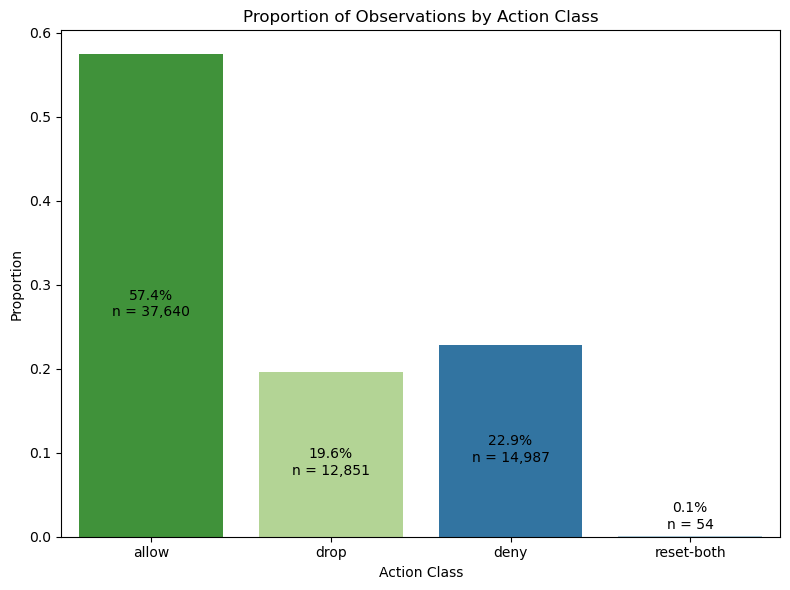
\includegraphics[width=0.60\textwidth]{figures/target_distribution.png}
    \caption{Proportion of observations in each action class. Counts and percentages are labeled on or above the bars.}
	\label{fig:target_distribution}
\end{figure}

\subsection{Preprocessing}

The dataset contains no missing values.

To better understand the port-related features and guide grouping decisions, the 20 most frequent values for each port column---\texttt{Source Port}, \texttt{NAT Source Port}, \texttt{Destination Port}, and \texttt{NAT Destination Port}---were plotted, stratified by action class. As shown in Figure~\ref{fig:frequent_ports}, several class-specific patterns are noticeable.

\begin{itemize}
    \item \texttt{allow} traffic is dominant on service ports like 80 (HTTP), 443 (HTTPS), and 53 (DNS), especially in \texttt{Destination Port} and \texttt{NAT Destination Port}.
    \item \texttt{deny} and \texttt{drop} actions are more common on remote-access or vulnerable services such as ports 22 (SSH), 23 (Telnet), 445 (SMB), and 5900 (VNC).
    \item Port 443 appears in \texttt{Source Port} more often with \texttt{deny} than \texttt{allow} actions---an unusual pattern, as this port is typically seen in the \texttt{Destination Port} field for HTTPS traffic.
    \item Port 0 frequently appears in \texttt{NAT Source Port} and \texttt{NAT Destination Port} among \texttt{deny}, \texttt{drop}, and \texttt{reset-both} classes, suggesting anonymized or missing NAT data.
    \item Ephemeral source ports ($\geq$1024)with low frequency dominate \texttt{allow} traffic in \texttt{Source Port}.
\end{itemize}

Interestingly, all rows with \texttt{Action = drop} had \texttt{NAT Destination Port = 0}. Nearly all \texttt{deny} and \texttt{reset-both} rows showed the same. Most \texttt{allow} rows had matching NAT and non-NAT destination ports---except for 480 cases, 479 of which had \texttt{NAT Destination Port = 0}.

Each of the four port features had a large number of unique values, many of which were rare. To reduce the dimensionality introduced by one-hot encoding and to keep the total number of model features under approximately 1000 (especially important for the RBF SVM), low-frequency values were grouped into a single \texttt{infrequent} category. Thresholds were set individually: a stricter cutoff of 10 was used for \texttt{Source Port}, and a threshold of 5 for the other three features.

The decision to group aggressively on \texttt{Source Port} was also supported by domain knowledge: high-numbered ports ($\geq$1024), which dominate this feature, typically correspond to ephemeral outbound client-side connections. These ports are common in \texttt{allow} traffic and tend to have high cardinality but low frequency---that is, wide variety with shallow support. While this grouping labeled nearly 87\% of \texttt{Source Port} values as \texttt{infrequent}, it drastically reduced feature count while preserving patterns in the data.

\begin{figure}[H]
	\centering
	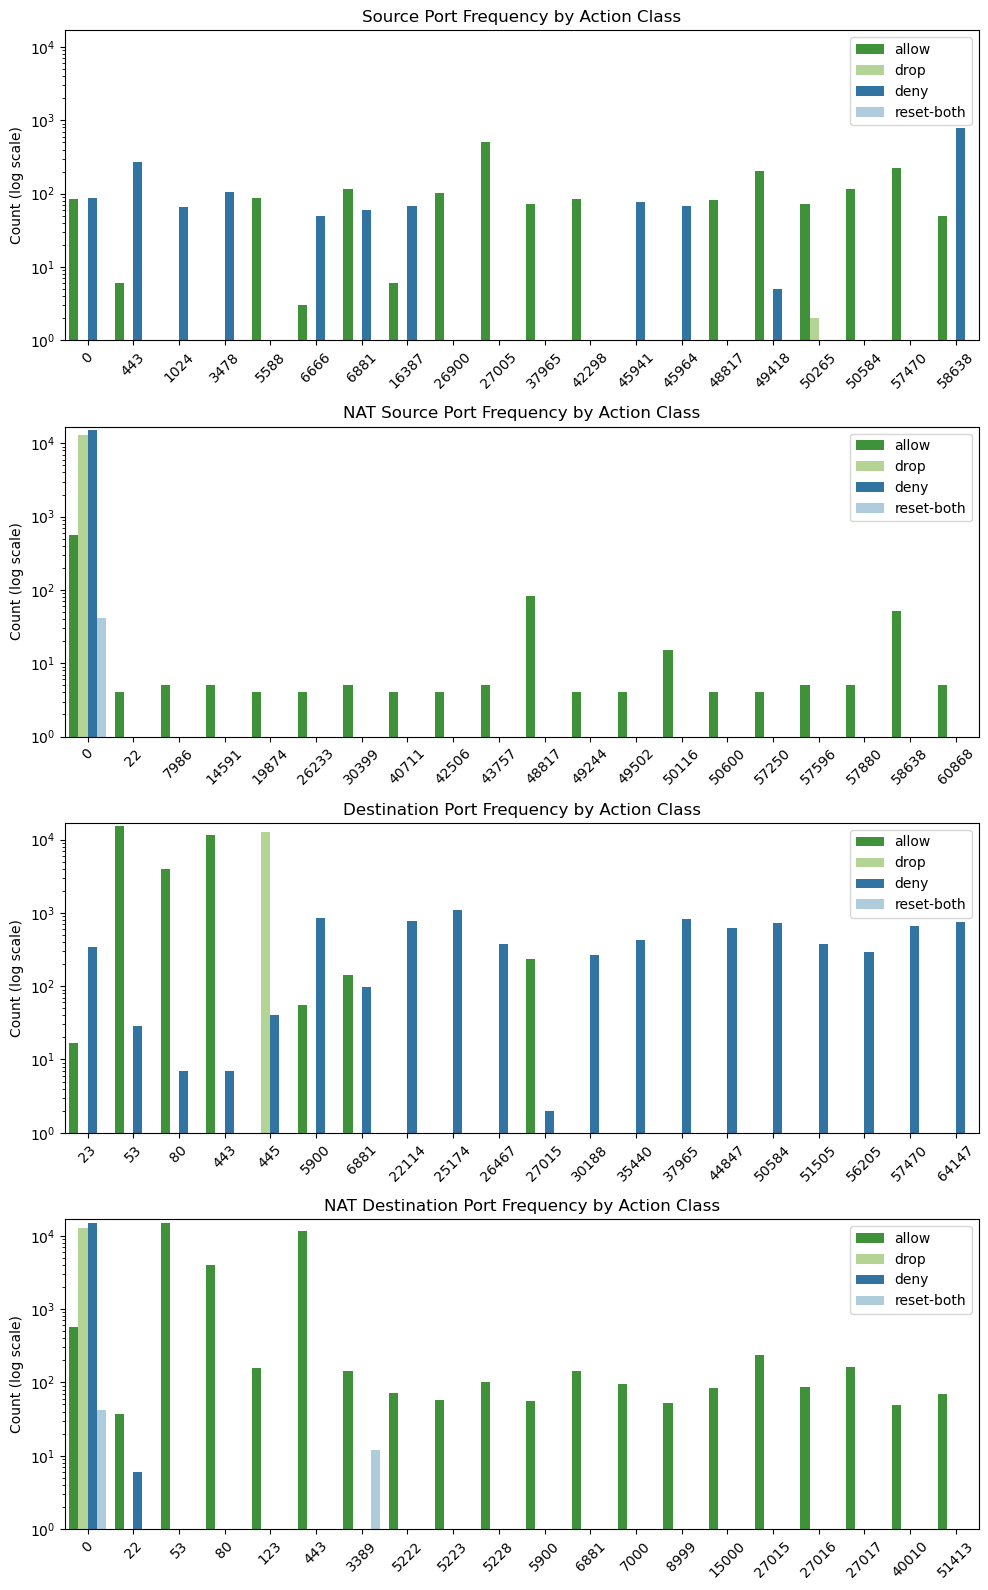
\includegraphics[width=0.84\textwidth]{figures/frequent_ports.png}
	\captionsetup{width=0.84\textwidth}
	\caption{Barplot of the top 20 most frequent values for each port-related feature, stratified by \texttt{Action} class. Frequencies are displayed on a log scale to account for the wide range and skewed distribution of port usage counts.}
	\label{fig:frequent_ports}
\end{figure}

Table~\ref{table:port_reduction} summarizes the observation thresholds, original and reduced category counts, and the percentage of rows labeled \texttt{infrequent} for each port feature.

\begin{table}[!h]
    \centering
    \caption{Port Feature Reduction via Infrequent Grouping}
    \begin{tabular}{lrrrr}
    \arrayrulecolor{black}  % Start with black rules
    \toprule
    \textbf{Port Feature} & \textbf{Threshold} & \textbf{Original Categories} & \textbf{After Grouping} & \textbf{\% Infrequent Rows} \\
    \midrule
    \arrayrulecolor{lightgray}
    Source Port           & 10 & 22{,}724 & 404  & 86.92\% \\ \hline
    NAT Source Port       & 5  & 29{,}152 & 12   & 56.33\% \\ \hline
    Destination Port      & 5  & 3{,}273  & 374  & 7.03\%  \\ \hline
    NAT Destination Port  & 5  & 2{,}533  & 110  & 5.79\%  \\
    \arrayrulecolor{black}
    \bottomrule
    \end{tabular}
    \label{table:port_reduction}
\end{table}

After grouping infrequent values, the categorical values in each of the four port-related features were one-hot encoded, with the first category dropped as a reference level.

The numeric features were log-transformed because of extreme skewness in their distributions. Figure~\ref{fig:log_distributions} shows the distributions of \texttt{Bytes}, \texttt{Packets}, and \texttt{Elapsed Time (sec)} by action class after log transformation. While log transformation reduced skewness, the distributions remained non-normal.

\begin{figure}[!h]
	\centering
	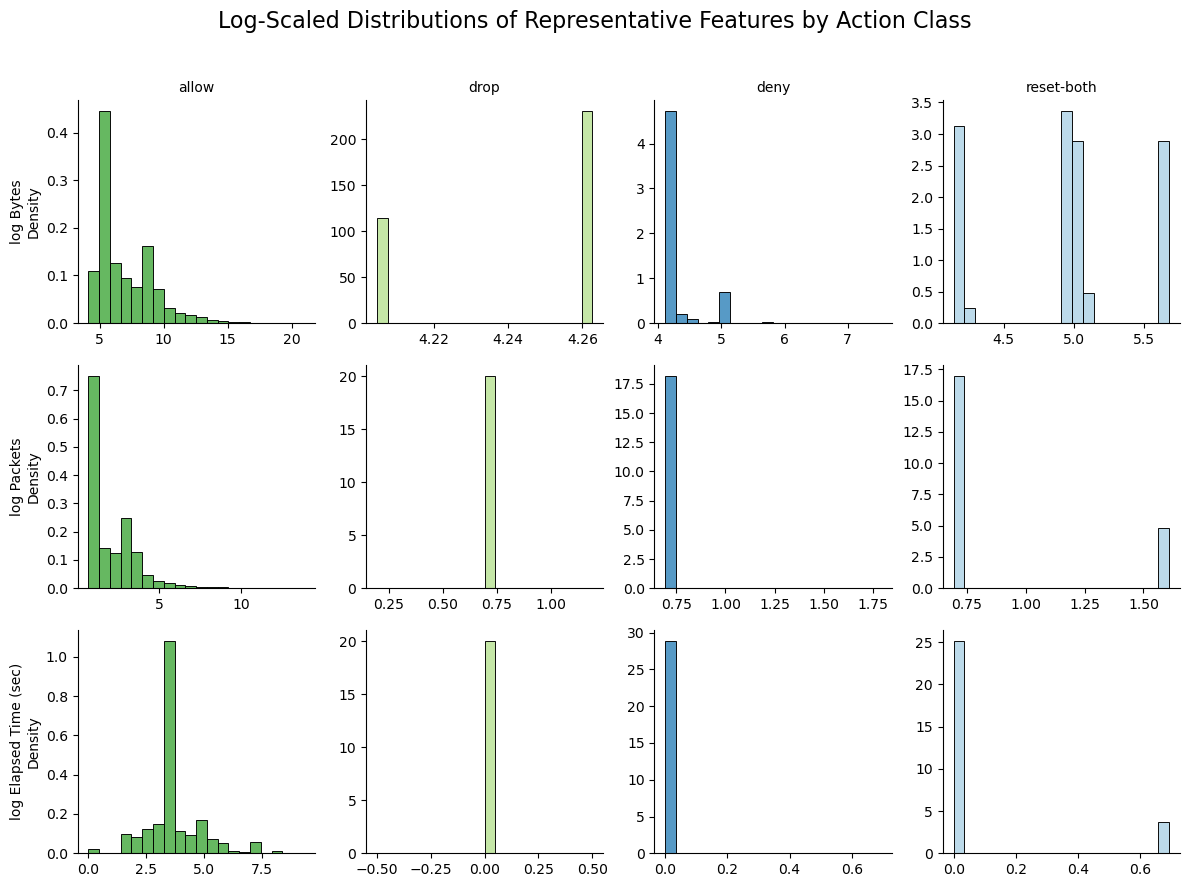
\includegraphics[width=0.95\textwidth]{figures/log_distributions.png}
	\caption{Histograms of representative features \texttt{Bytes}, \texttt{Packets}, and \texttt{Elapsed Time (sec)} for each action class after log transformation. Log transformation reduced the skewness of the distributions, but they remained non-normal.}
	\label{fig:log_distributions}
\end{figure}

The log-transformed features were then scaled using \texttt{StandardScaler}. Scaling is important for SVM and SGD-based logistic regression because both are sensitive to feature magnitudes. SVM maximizes the margin based on Euclidean distances, so features with larger ranges can distort the decision boundary. In SGD, weight updates depend on the scale of the inputs, and scaling ensures that all features contribute proportionally during training.

\section{Modeling}

\subsection{Linear SVM}

Scikit-Learn's \texttt{LinearSVC()} was used to build a linear support vector machine (SVM) model with L2 regularization and a squared-hinge loss function. The \texttt{class\_weight='balanced'} option was specified to account for class imbalance in the target.

The regularization parameter \texttt{C} was tuned over 20 logarithmically spaced values from \texttt{1e-6} to \texttt{1e6} using 5-fold stratified and shuffled cross-validation. A value of \texttt{C = 2.07} was selected because it achieved similarly high accuracy to nearby values, while providing stronger regularization and faster computation. Slightly higher accuracy (within one standard deviation) was observed at larger values of \texttt{C}, but this came at the cost of longer training time and weaker regularization.

To evaluate the model, \texttt{cross\_val\_predict()} was used with stratified and shuffled 5-fold cross-validation and the selected \texttt{C} value. This produced out-of-fold predictions used to generate a classification report and confusion matrix.

\subsection{Nonlinear SVM (RBF Kernel)}

A nonlinear SVM model was built using \texttt{SVC()} with an RBF kernel, which applies the kernel trick to map inputs into a higher-dimensional space. As before, the \texttt{class\_weight='balanced'} option was used to address class imbalance in the target. A cache size of 400 (double the default of 200) was set to improve model training speed.

The regularization parameter \texttt{C} was tuned over the same parameter space, ranging from \texttt{1e-6} to \texttt{1e6}, but instead of cross-validation, a single 80/20 stratified and shuffled train/test split was used to reduce computational cost. A value of \texttt{C = 5.46e4} was selected because it achieved the highest accuracy and fastest computation among all tested values, while also providing stronger regularization than other models with comparable accuracy.

Model performance was evaluated on the 20\% holdout test set using a classification report and a confusion matrix.

\subsection{SGD Logistic Regression}

\texttt{SGDClassifier()} with \texttt{loss='log\_loss'} was used to build a logistic regression model with L2 regularization, trained using Stochastic Gradient Descent. As before, the \texttt{class\_weight='balanced'} option was used to address class imbalance in the target.

The penalty term \texttt{alpha} was tuned in two stages: a coarse grid from \texttt{1e-6} to \texttt{1e0}, and a fine grid from \texttt{1e-5} to \texttt{1e-3}, both using 5-fold stratified and shuffled cross-validation. The best value, \texttt{alpha = 2.15e-4}, achieved the highest mean accuracy and lowest standard deviation with comparable training time.

The default maximum number of epochs (\texttt{max\_iter=1000}) was used with \texttt{early\_stopping=True} and a stopping criterion of 10 epochs without improvement (\texttt{n\_iter\_no\_change=10}). The loss was evaluated on 20\% of the shuffled CV training data (\texttt{validation\_fraction=0.2}, \texttt{shuffle=True}). Using the selected \texttt{alpha}, along with \texttt{learning\_rate='optimal'} and \texttt{tol=0.001}, the model converged in 11 epochs. Although the loss decreased slightly beyond epoch 1, it did not decrease beyond the tolerance threshold, triggering early stopping.

To encourage convergence in the 20-100 epoch range, \texttt{tol} values from \texttt{1e-3} to \texttt{1e-5} were tested. Accuracy remained stable, and average epochs increased only slightly, so the default tolerance was retained.

Learning rate strategies were also tested: \texttt{learning\_rate='optimal'} versus \texttt{learning\_rate='adaptive'} with \texttt{eta0} ranging from \texttt{1e-5} to \texttt{1e-1}. The best adaptive model used \texttt{eta0 = 1e-2} and trained for 106 epochs, aligning with the target range.

To select the final SGD model, both learning rate strategies were evaluated using \texttt{alpha = 2.15e-4} and \texttt{tol = 0.001}, with the \texttt{adaptive} model using the tuned \texttt{eta0 = 1e-2}.

\vspace{0.5em}
\noindent
Comparison of learning rate strategies for the SGD logistic regression model:
\begin{itemize}
  \item Optimal LR: Log loss = 0.0341 $\pm$ 0.0055, accuracy = 0.9966 $\pm$ 0.0004, 11 epochs, avg. time = 0.151s
  \item Adaptive LR: Log loss = 0.0415 $\pm$ 0.0006, accuracy = 0.9968 $\pm$ 0.0002, 71 epochs, avg. time = 0.613s
\end{itemize}
\noindent

The adaptive LR was slower and had slightly higher loss. For simplicity and efficiency, the default \texttt{optimal} setting was selected.

\subsection{Parameter Summary}

The key hyperparameters for each final model are summarized in Table~\ref{table:key_params}.

\begin{table}[h!]
    \centering
    \caption{Final Hyperparameters for Each Selected Model}
    \begin{tabular}{ll}
    \arrayrulecolor{black}
    \toprule
    \textbf{Model} & \textbf{Key Hyperparameters} \\
    \midrule
    Linear SVM (\texttt{LinearSVC()}) & \texttt{C = 2.07}, \\
    & \texttt{loss='squared\_hinge'}, \\
    & \texttt{penalty='l2'} \\
    \midrule
    RBF SVM (\texttt{SVC()}) & \texttt{C = 5.46e4}, \\
    & \texttt{kernel='rbf'} \\
    \midrule
    SGD Logistic Regression (\texttt{SGDClassifier()}) & \texttt{alpha = 2.15e-4}, \\
    & \texttt{loss='log\_loss'}, \\
    & \texttt{learning\_rate='optimal'}, \\
    & \texttt{early\_stopping=True}, \\
    & \texttt{tol=0.001}, \\
    & \texttt{n\_iter\_no\_change=10} \\
    \bottomrule
    \end{tabular}

    \vspace{0.5em}
        \small\textit{Note: All models were trained with \texttt{class\_weight='balanced'} to address class imbalance.}
    \label{table:key_params}
\end{table}

\section{Results}

\subsection{Confusion Matrices}

To generate the confusion matrices shown in Figure~\ref{fig:confusion_matrices}, a default classification threshold of 0.5 was used for all models. Each matrix is shown with raw counts on the left and normalized values on the right to facilitate comparison between cross-validated and holdout models.

All three models achieved near-perfect accuracy on the \texttt{allow} class. For the two SVM models, fewer than 0.1\% of \texttt{allow} observations were misclassified as \texttt{deny}, while the SGD model misclassified 0.27\% as \texttt{deny} and fewer than 0.1\% as \texttt{reset-both}.

The \texttt{deny} class was also classified with high accuracy---between 98\% and nearly 100\%---across all models. Fewer than 0.1\% of \texttt{deny} observations were mislabeled as \texttt{allow}, with the remaining misclassifications split between \texttt{drop} and \texttt{reset-both}.

All three models perfectly predicted the \texttt{drop} class, with no misclassifications.

The minority class \texttt{reset-both}, which made up only 0.1\% of the dataset (54 examples), was the most frequently misclassified. All misclassifications were as \texttt{deny}. The linear SVM and RBF SVM misclassified 22\% and 27\%, respectively, while the SGD model misclassified 48\%.

\begin{figure}[H]
	\centering
	
\includegraphics[width=1.0\textwidth]{figures/confusion_matrices.png}
	\caption{Confusion matrices showing classification results for the linear SVM (top row, green), RBF SVM (middle row, blue), and SGD logistic regression (bottom row, purple) models. Raw counts are shown on the left and normalized values on the right.}
	\label{fig:confusion_matrices}
\end{figure}

\subsection{Overall Metrics}

All three models achieved similarly high accuracy, as shown in Table~\ref{table:metrics_overall}, with linear SVM (0.9981 $\pm$ 0.0002) and SGD logistic regression (0.9966 $\pm$ 0.0004) exhibiting slightly higher and more stable performance across cross-validation folds compared to the RBF SVM (0.9946), which was evaluated on a single holdout test set.

Macro-averaged metrics evaluate performance across all classes equally, giving the same weight to minority classes regardless of their frequency. In contrast, weighted metrics adjust for class frequency when averaging across classes. Whether macro or weighted metrics are more appropriate depends on the analytic goal, whether to prioritize minority classes or overall dataset performance.

The linear SVM achieved the highest macro and weighted scores overall, reflecting the strongest and most consistent performance across all classes. As expected, the SGD logistic regression model ran faster than either SVM model, with the RBF SVM being the slowest. The SGD model outperformed the RBF SVM in all metrics except for macro recall and weighted precision. The macro metrics tend to be lower than the weighted metrics due to lower performance on the minority class, \texttt{reset-both}.

\begin{table}[h!]
    \centering
    \caption{Overall Classification Metrics and Modeling Time by Model}
    \begin{tabular}{lccc}
    \arrayrulecolor{black}
    \toprule
    \textbf{Metric} & \textbf{Linear SVM (CV)} & \textbf{RBF SVM (Holdout)} & \textbf{SGD Logistic Regression (CV)} \\
    \midrule
    \arrayrulecolor{lightgray}
    Accuracy              & 0.9981 & 0.9946 & 0.9966 \\
    Macro Precision       & 0.8848 & 0.7799 & 0.8485 \\
    Macro Recall          & 0.9429 & 0.9263 & 0.8777 \\
    Macro F1-score        & 0.9088 & 0.7999 & 0.8614 \\
    Weighted Precision    & 0.9983 & 0.9981 & 0.9968 \\
    Weighted Recall       & 0.9981 & 0.9946 & 0.9966 \\
    Weighted F1-score     & 0.9982 & 0.9961 & 0.9967 \\
    Modeling Time (s)     & 0.37   & 0.84   & 0.18 \\
    \arrayrulecolor{black}
    \bottomrule
    \end{tabular}
    \vspace{0.5em}
    \caption*{\small\textit{Note: Modeling times include both training and prediction. Times for cross-validated models reflect the mean per fold. RBF SVM time is based on a single train/test split.}}
    \label{table:metrics_overall}
\end{table}
   
\subsection{Per-Class Metrics}

As shown in Table~\ref{table:metrics_by_class}, all models achieved at least 99.5\% precision, recall, and F1-score on the \texttt{allow} and \texttt{drop} classes. The linear SVM also reached at least 99.5\% on all three metrics for the \texttt{deny} class.

For \texttt{deny}, the RBF SVM showed the highest precision (99.8\%) but lower recall (97.8\%) and F1-score (98.8\%) than the other models. The SGD model had slightly lower precision (99.2\%) but higher recall (99.6\%).

The minority class \texttt{reset-both} was the most challenging for all models. The linear SVM achieved the best performance: precision (54.6\%), recall (77.8\%), and F1-score (64.1\%). The SGD model lagged behind the others models with lower recall of 51.9\%, while the RBF SVM showed very low precision (12.5\%) despite a relatively high recall (72.7\%).

\begin{table}[H]
    \centering
    \caption{Per-Class Classification Metrics for Each Model}
    \begin{tabular}{llrrrr}
    \arrayrulecolor{black}
    \toprule
    \textbf{Model} & \textbf{Class} & \textbf{Precision} & \textbf{Recall} & \textbf{F1-score} & \textbf{Support} \\
    \midrule
    Linear SVM (CV) & & & & & \\
    & allow       & 0.9999 & 0.9992 & 0.9995 & 37{,}640 \\
    & deny        & 0.9971 & 0.9947 & 0.9959 & 14{,}987 \\
    & drop        & 0.9969 & 1.0000 & 0.9984 & 12{,}851 \\
    & reset-both  & 0.5455 & 0.7778 & 0.6412 & 54 \\
    \midrule
    RBF SVM (Holdout) & & & & & \\
    & allow       & 1.0000 & 0.9996 & 0.9998 & 7{,}528 \\
    & deny        & 0.9980 & 0.9783 & 0.9880 & 2{,}998 \\
    & drop        & 0.9965 & 1.0000 & 0.9983 & 2{,}570 \\
    & reset-both  & 0.1250 & 0.7273 & 0.2133 & 11 \\
    \midrule
    SGD Logistic Regression (CV) & & & & & \\
    & allow       & 0.9997 & 0.9966 & 0.9982 & 37{,}640 \\
    & deny        & 0.9916 & 0.9955 & 0.9935 & 14{,}987 \\
    & drop        & 0.9969 & 1.0000 & 0.9984 & 12{,}851 \\
    & reset-both  & 0.4058 & 0.5185 & 0.4553 & 54 \\
    \bottomrule
    \end{tabular}
\label{table:metrics_by_class}
\end{table}

\section{Conclusion}

All three models achieved high accuracy, as well as strong precision, recall, and F1-scores across most classes---except for the minority class, \texttt{reset-both}, which was challenging for all. Because both linear models produced slightly better overall metrics and ran more quickly, the results suggest that a linear model is sufficient for this application.

The linear SVM was slightly slower than the SGD model, but it achieved the highest overall accuracy and the best per-class metrics, including on the \texttt{reset-both} class. It was also the easiest model to tune. Given the size of this dataset, either linear model would be a strong choice for optimizing performance. However, with larger datasets, the SGD model would likely offer a better balance of speed, scalability, and performance.

\end{document}
